\documentclass{ctexart}
\usepackage{xcolor}
\usepackage{graphicx}
\usepackage{mathtools}
\usepackage{amssymb}
\usepackage[colorlinks, linkcolor=red]{hyperref}
\begin{document}

	\section{概论}
	
	\subsection{统计学习}
	
	统计学习方法三要素:模型、策略、算法
	
	统计学习(statistical learning):关于计算机基于数据构建概率统计模型并运用模型对数据进行预测和分析的一门学科
	
	统计学习由监督学习(supervised learning)、非监督学习(unsupervised learning)、半监督学习(semi-supervised learning)、强化学习(reinforcement learining)等组成
	
	监督学习下统计学习步骤可以概括为:
	
	1.得到一个有限的训练数据集合(training data)
	
	2.确定包含所有可能的模型的假设空间(hypothesis space),即学习模型的组合
	
	3.确定模型选择的准则,即学习的策略
	
	4.实现求解最优模型的算法,即学习的算法
	
	5.通过学习方法选择最优模型
	
	6.利用学习的最优模型对新数据进行预测或分析

	\subsection{监督学习}
	
	在监督学习中,将输入与输出所有可能取值的集合分别称为输入空间(input space)和输出空间(output space)
	
	每个具体的输入时一个实例(instance),通常由特征向量(feature vector)表示。所有特征向量存在的空间称为特征空间(feature space)。特征空间的每一维对应于一个特征。输入空间与特征空间不一定相同,有时候需要将输入空间映射至特征空间(比如图片,音频)。{\color{red}模型实际上都是定义在特征空间上。}
	
	输入输出变量用大写字母表示,输入输出变量所取的值用小写字母表示。输入实例\(x\)的特征向量记作:
	
	\[x=(x^{(1)}, x^{(2)}, ..., x^{(i)}, ... x^{(n)})^T\]
	
	\(x^{(i)}\)表示\(x\)的第i个特征向量,\(x^{(i)}\)与\(x_i\)不同,\(x_i\)表示多个输入变量中的第i个,即
	
	\[x=(x^{(1)}_i, x^{(2)}_i, ..., x^{(n)}_i)^T\]
	
	监督学习从训练数据集合中学习模型,对测试数据进行预测。训练数据由输入与输出对组成,通常表示成:
	
	\[T=\{(x_1,y_1),(x_2,y_2),...,(x_N,y_N)\}\]
	
	监督学习假设输入与输出的随机变量X和Y遵循联合概率分布P(X,Y)。P(X,Y)表示分布函数或分布密度函数。在学习过程中,假定这一联合概率分布存在。统计学习假设数据存在一定的统计规律,{\color{red}X和Y具有联合概率分布的假设就是监督学习关于数据的基本假设。}
	
	监督学习的目的在于学习一个由输入到输出的映射,这一映射由模型来表示。模型属于由输入空间到输出空间的映射的集合,这个集合就是假设空间。假设空间的确定意味着学习范围的确定。
	
	监督学习氛围学习和预测两个过程。
	
	\begin{center}
		%\centering
		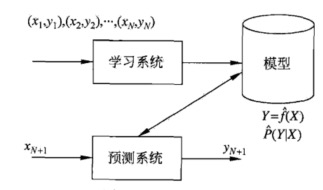
\includegraphics[width=0.8\linewidth]{pic/supervised_learning_problem}
		%\caption[监督学习问题]{}
		\label{fig:supervised-learning-problem}
	\end{center}

	\subsection{统计学习三要素}
	
	\textbf{模型}:在监督学习中,模型就是所要学习的条件概率分布(为什么是条件概率分布?可以理解为在已知数据的情况下模型的可能性)或决策函数。模型的假设空间包含所有可能的条件概率分布或决策函数。例如,假设决策函数是输入变量的线性函数,那么模型的假设空间就是所欲这些线性函数构成的函数集合。假设空间的模型一般有无穷多个。
	
	假设空间用F表示,假设空间可以定义为决策函数的集合
	
	\[F=\{f|Y=f(X)\}\]
	
	其中X和Y是定义在输入空间X和输出空间Y上的变量。这时F通常是由一个参数向量决定的函数族:
	
	\[F=\{f|Y=f_\theta(X), \theta \in R^n\}\]
	
	参数向量\(\theta\)取决于n为欧氏空间\(R^n\),称为参数空间
	
	假设空间也可以定义为条件概率的集合
	
	\[F=\{P|P(Y|X)\}\]
	
	其中X和Y是定义在输入空间X和输出空间Y上的随机变量,这时F通常是由一个参数向量决定的条件概率分布族:
	
	\[F=\{P|P_\theta(Y|X), \theta \in R^n\}\]
	
	参数向量\(\theta\)取决于n为欧氏空间\(R^n\),称为参数空间
	
	\mbox{}
	
	\textbf{策略}:从假设空间中选择最优模型。
	
	1.损失函数和风险函数
	
	用一个损失函数或代价函数来度量预测错误的成都
	
	常用的损失函数有:
	
	(1)0-1损失函数(0-1 loss function)
	
	\[L(Y, f(X)) = 
	\begin{dcases}
	1,  & Y \neq f(X) \\
	0, & Y = f(X)
	\end{dcases}\]
	
	(2)平方损失函数(quadratic loss function)
	
	\[L(Y, f(X)) = (Y-f(X))^2\]
	
	(3)绝对损失函数(absolute loss funtion)
	
	\[L(Y, f(X)) = |Y - f(X)|\]
	
	
	(4)对数损失函数(logarithmic loss function)
	
	\[L(Y, P(Y|X)) = -logP(Y|X)\]
	
	损失函数值越小,模型越好,由于模型的输入、输出(X,Y)是随机变量,遵循联合分布P(X,Y),所以损失函数的期望
	
	\[R_{exp}(f) = E_p[L(Y, f(X))] = \int L(y, f(x))P(x, y)dxdy\]
	
	该表达式成为风险函数(risk function)或期望损失(expected loss)
	
	给定一个训练集,模型f(X)关于训练数据集的平均损失成为经验风险(empirical risk)或经验损失。
	
	\[R_{emp}(f) = \frac{1}{N}\sum_{i=1}^{N}L(y_i, f(x_i))\]
	
	期望风险\(R_{exp}(f)\)是模型关于联合分布的期望损失,经验风险\(R_{emp}(f\))是模型关于训练样本集的平均损失。根据大数定律,当样本容量N趋于无穷,经验风险趋于期望风险。
	
	现实中,训练数据集有限,所以经验风险估计期望风险并不理想,所以需要矫正。监督学习中有两个基本策略:经验风险最小化和结构风险最小化。
	
	在假设空间,损失函数和训练数据集确定的情况下,经验风险函数式就可以确定。经验风险最小化(empirical risk minimazation, ERM)的策略认为,经验风险最小的模型就是最优模型。比如极大似然估计。{\color{red}当模型是条件概率分布,损失函数是对数损失函数时,经验风险最小化就等价于极大似然估计}
	
	(\textbf{思考:极大似然估计与贝叶斯估计在机器学习中的应用以及跟损失函数这些有没有什么联系?}数理统计中的极大似然估计以及贝叶斯估计也只是估计模型参数的一种策略,极大似然估计针对的是条件概率分布的情况下,损失函数是对数损失函数,可以联系概率统计中是怎么计算极大似然估计的。)
	
	\[\min_{f \in F} \frac{1}{N} \sum_{i=1}^{N}L(y_i, f(x_i))\]
	
	样本容量很小时,经验风险最小化学习的效果就不是很好,就容易出现过拟合现象。结构风险最小化(structural risk minimization, SRM)是为了防止过拟合而提出来的策略。结构风险最小化等价于正则化(regularization)。结构风险最小化在经验风险上加上表示模型复杂度的正则化项(regularizer)或罚项(penalty term)。
	
	\[R_{emp}(f) = \frac{1}{N}\sum_{i=1}^{N}L(y_i, f(x_i)) + \lambda J(f)\]
	
	J(f)为模型的复杂度,是定义在假设空间F上的泛函。模型f越复杂,复杂度越大。复杂度表示了对复杂模型的惩罚。\(\lambda \geq 0\)是系数,用以权衡经验风险和模型复杂度。结构风险小需要经验风险和复杂度同时小。
	
	结构风险最小化策略认为结构风险最小的模型是最优模型。即:
	
	\[\min_{f \in F}  \frac{1}{N} \sum_{i=1}^{N}L(y_i, f(x_i)) + \lambda J(f)\]
	
	这样监督学习问题就变成了经验风险或结构风险函数的最优化问题。这时,经验或结构风险函数是最优化的目标函数。
	
	\mbox{}
	
	\textbf{算法}:是指学习模型的具体计算方法。统计学习基于训练数据集,根据学习策略,从假设空间中选择最优模型,然后考虑用什么计算方法求解最优模型。这时,统计学习问题归结为最优化问题,统计学习的算法成为求解最优化问题的算法。
	
	\mbox{}
	
	\textbf{总结:}
	
	1.模型:根据数据的分布情况,选定模型,目的是找出模型的参数
	
	2.策略:根据情况选定损失函数(0-1,平均,绝对,对数),目标就是让损失函数最小
	
	3.算法:初始化参数,根据不同的算法(比如梯度下降)来修正模型的参数,使损失函数最小

	\subsection{模型的评估与模型选择}
	
	假设学习到的模型是\(Y = \hat{f}(X)\),训练误差是模型\(Y = \hat{f}(X)\)关于训练集的平均损失。
	
	\[R_{emp}(\hat{f}) = \frac{1}{N}\sum_{i=1}^{N}L(y_i, \hat{f}(x_i))\]
	
	其中N是训练样本容量。
	
	测试误差是模型\(Y = \hat{f}(X)\)关于测试数据集的平均损失:
	
	\[e_{test} = \frac{1}{N^{'}}\sum_{i=1}^{N^{'}}L(y_i, \hat{f}(x_i))\]
	
	其中\(N^{'}\)是测试样本容量
	
	训练误差的大小,本质上不重要,但测试误差反映了学习方法对未知数据集的预测能力,是重要的。测试误差小的方法具有更好地预测能力。
	
	所选择的模型的参数向量与真模型的参数向量接近。如果一味追求提高对训练数据的预测能力,所选模型的复杂度往往会比真模型更高,这就是过拟合现象(over-fitting)。过拟合是指学习时选择的模型所包含的参数过多,以致于出现这一模型对已知数据预测得很好,但对位置数据预测得很差的现象。
	
	\begin{center}
	%\centering
	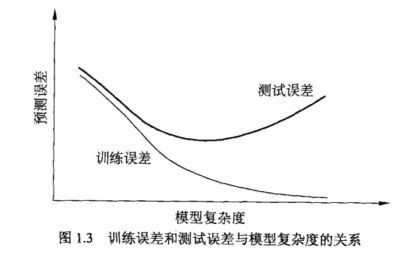
\includegraphics[width=0.8\linewidth]{pic/training_error_and_testing_error}
	\end{center}

	\subsection{模型选择的方法}
	
	模型选择的典型方法是正则化。正则化项一般是模型复杂度的单调递增函数,模型越复杂,正则化值就越大。比如,正则化项可以是模型参数向量的范数。
	
	\[\min_{f \in F}  \frac{1}{N} \sum_{i=1}^{N}L(y_i, f(x_i)) + \lambda J(f)\]
	
	正则化的作用是选择经验风险与模型复杂度同时比较小的模型
	
	奥卡姆剃刀(Occam's razor)原理应用于模型选择时,在所有的可能选择的模型中,能够很好地解释已知数据并且十分简单的才是最好的模型。
	
	从贝叶斯估计的角度看,正则化项对应于模型的先验概率。可以假设复杂的模型有较小的先验概率,简单的模型有较大的先验概率。
	
	另一种常用的模型选择方法是交叉验证(cross validation)。
	
	如果给定的样本数据充足,进行模型选择的一种简单方法就是随机地将数据集切成三部分,分别为训练集,验证集和测试集。训练集用来训练模型,验证集用于模型的选择,而测试集用于最终对学习方法的评估。
	
	1. 简单交叉验证:随机地将已给数据分为两个部分,一部分作为训练集,另一部分作为测试集。
	
	2. S折交叉验证: 首先随机地将已给数据切分为S个互不相交的大小相同的子集;然后利用S-1个子集的数据训练模型,利用余下的子集测试模型;将这一过程对可能的S中选择重复进行;最后选出S次评测中平均测试误差最小的模型
	
	3.留一交叉验证:S折交叉验证的特殊情形是S=N,N是给定数据集的容量

	\subsection{泛化能力}
	
	学习方法的泛化能力(generalization ability)是指该方法学习到的模型对未知数据的预测能力。
	
	如果学到的模型师\(\hat(f)\),那么这个模型对未知数据预测的误差,即泛化误差。
	
	\[R_{exp}(f) = E_p[L(Y, f(X))] = \int_{X\times Y} L(y, f(x))P(x, y)dxdy\]
	
	泛化误差反映了学习方法的泛化能力,如果一种方法学习的模型比另一种方法学习的模型具有更小的泛化误差,那么这种方法更有效。泛化误差就是所学到的模型的期望风险。
	
	学习方法的泛化能力分析往往是通过研究泛化误差的概率上界进行的,简称泛化误差上界(generalizaiton error bound)。泛化误差上界具有以下性质:它是样本容量的函数,当样本容量增加时,泛化上界趋近于0;它是假设空间容量的函数,假设空间容量越大,模型越难学,泛化误差上界越大。
	
	\textbf{定理:泛化误差上界:} 对二分类问题,当假设空间是有限个函数的集合\(F = \{f_1, f_2,...,f_d\}\)时,对任意一个函数\(f \in F\),至少以概率\(1-\delta\),以下不等式成立:
	
	\[R(f) \leq \hat{R}(f) + \varepsilon(d, N, \delta)\]
	
	其中:
	
	\[\varepsilon(d, N, \delta) = \sqrt{\frac{1}{2N}(log d + log\frac{1}{\delta})}\]
	
	不等式左端R(f)是泛化误差,右端是泛化误差上界。在泛化误差上界中,第一项是训练误差,训练误差越小,泛化误差也越小,第二项是N的单调递减函数,当N趋于无穷大时趋于0;同时它也是\(\sqrt{logd}\)的函数,假设空间F所包含的函数越多,其值越大。

	\mbox{}

	\textbf{补充:最大似然估计与贝叶斯估计}
	
	极大似然估计与贝叶斯估计是统计中两种对模型的参数确定的方法,两种参数估计方法使用不同的思想。前者来自于频率派,认为参数是固定的,我们要做的事情就是根据已经掌握的数据来估计这个参数;而后者属于贝叶斯派,认为参数也是服从某种概率分布的,已有的数据只是在这种参数的分布下产生的。所以,直观理解上,极大似然估计就是假设一个参数\(\theta\),然后根据数据来求出这个\(\theta\). 而贝叶斯估计的难点在于p(\(\theta\)) 需要人为设定,之后再考虑结合MAP(maximum a posterior)方法来求一个具体的θ. 
	
	
	所以极大似然估计与贝叶斯估计最大的不同就在于是否考虑了先验,而两者适用范围也变成了:{\color{red}极大似然估计适用于数据大量,估计的参数能够较好的反映实际情况;而贝叶斯估计则在数据量较少或者比较稀疏的情况下,考虑先验来提升准确率}。

	
	\url{https://sine-x.com/statistical-learning-method/}

	\section{感知机}
	
	感知机(percetron)是二类分类的线性分类模型,其输入为实例的特征向量,输出为实例的类别,取+1和-1二值。感知机对应于输入空间中将实例划分为正负两类的分离超平面,属于判别模型。
	
	感知机学习旨在求出将训练数据进行线性化分的分离超平面,为此,导入基于误分类的损失函数,利用梯度下降法对损失函数进行极小化,求得感知机模型。

	\subsection{感知机模型}
	
	\textbf{定义:感知机} 假设输入空间(特征空间)是\(X \subseteq R^n\),输出空间是\(Y = \{+1, -1\}\)。输入\(x \in X\)表示实例的特征向量,对应于输入空间的点;输出\(y \in Y\)表示实例的类别。由输入空间到输出空间的如下函数成为感知机
	
	\[f(x) = sign(w·x + b)\]
	
	其中,w和b为感知机模型参数,\(w \in R^n\)叫做权值(weight)或权值向量(weight vector),\(b \in R\)叫做偏置(bias),w·x表示w和x的内积,sign是符号函数。
	
	\[sign(x) = 
	\begin{dcases}
	+1, & x \geq 0 \\
	-1, &  x < 0
	\end{dcases}\]
	
	感知机的假设空间是定义在特征空间中的所有线性分类模型(linear classification model)或线性分类器(linear classifier),即函数集合\(f|f(x) = w·x + b\)
	
	感知机的集合解释:线性方程
	\[w·x + b = 0\]
	对应于特征空间\(R^n\)中的一个超平面S,其中w是超平面的法向量,b是超平面的截距。这个超平面将特征空间划分为两部分,划分为正负两类。超平面S成为分离超平面(separating hyperplane)
	
	\begin{center}
		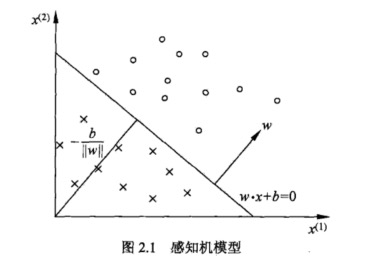
\includegraphics[width=0.8\linewidth]{pic/perceptron_model}
	\end{center}

	\subsection{感知机策略}
	
	数据集线性可分性:数据集的正实例和负实例能够被正确地划分到平面的两侧。
	
	如果训练数据集是线性可分的,感知机的学习目标就是求得一个能够将训练集正实例点和负实例点完全正确分开的分离超平面。
	
	损失函数采用的是误分类点到超平面S的总距离:
	
	\[\frac{1}{||w||}|w·x_0 + b|\]
	
	这里,\(||w||\)是w的\(L_2\)范数
	
	\textbf{证明:}如下图所示,O表示原点,Xp表示超平面上的一点,X是超平面外的一点,w是超平面的法向量。
	
	\begin{center}
	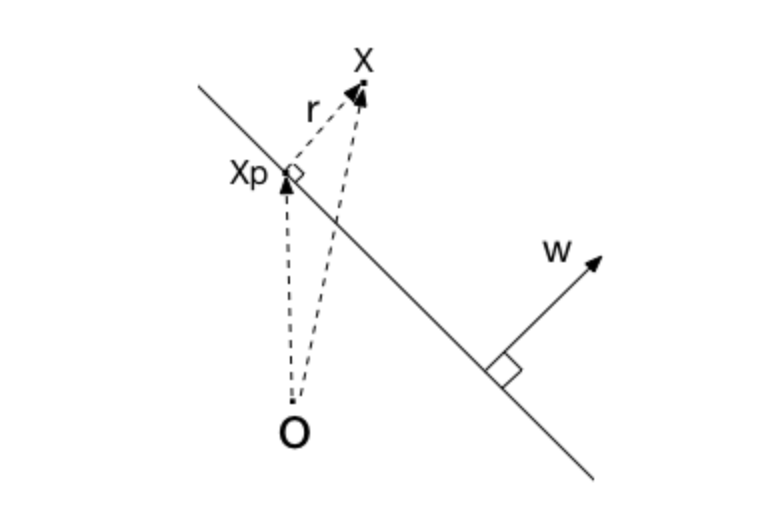
\includegraphics[width=0.8\linewidth]{pic/hyperplane}
	\end{center}
	
	向量的加法运算
	
	\[X = X_p + r · \frac{w}{||w||}\]
	
	将该式代入\(g(x) = w·x + b\)中得到
	
	\[g(x) = w^T(X_p + r · \frac{w}{||w||}) + b = (w^T·X_p + b) + w^T·r·\frac{w}{||w||} = r·||w||\]
	
	其中,因为\(X_p\)在超平面上,所以\(w·X_p + b = 0\),可得\(g(x) = r·||w||\)
	
	所以X到超平面的距离\(r = \frac{g(x)}{||w||}\)
	
	\url{https://blog.csdn.net/jaster_wisdom/article/details/78240949}
	
	\url{https://blog.csdn.net/lilyth_lilyth/article/details/8973972}
	
	梯度下降:一次将误分类集合中所有误分类点的梯度下降;
	
	随机梯度下降:随机选取一个误分类点使其梯度下降。	
	
	\mbox{}
	
	\textbf{补充:} 在数学上,范数包括向量范数和矩阵范数,向量范数表征向量空间中向量的大小,矩阵范数表征矩阵引起变化的大小。一种非严密的解释就是,对应向量范数,向量空间中的向量都是有大小的,这个大小如何度量,就是用范数来度量的,不同的范数都可以来度量这个大小,就好比米和尺都可以来度量远近一样;对于矩阵范数,学过线性代数,我们知道,通过运算AX=B,可以将向量X变化为B,矩阵范数就是来度量这个变化大小的。
	
	L2范数是我们最常见最常用的范数了,我们用的最多的度量距离欧氏距离就是一种L2范数,它的定义如下:
	
	\[||x||_2 = \sqrt{\sum_{i}x_i^2}\]
	
	表示向量元素的平方和再开平方。
	
	\url{https://blog.csdn.net/shijing_0214/article/details/51757564}
	
	\mbox{}
	
	对于误分类的数据\(x_i, y_i\)来说,
	
	\[-y_i(w·x_i + b) > 0\]

	因此误分类点\(x_i\)到超平面的距离就是
	
	\[-\frac{1}{||w||}y_i(w·x_i + b)\]	
	
	误分类点的总距离就是
	
	\[-\frac{1}{||w||}\sum_{x_i \in M}y_i(w·x + b)\]
	
	不考虑\(\frac{1}{||w||}\),就得到感知机学习的损失函数,定义为:
	
	\[L(w, b) = -\sum_{x_i \in M}y_i(w·x + b)\]
	
	其中M为误分类点的集合,该函数即为感知机学习的经验风险函数。
	
	损失函数非负,如果没有误分类点,损失函数值是0.而且误分类点越少,误分类点离超平面越接近,损失函数值就是越小。{\color{red}一个特定的样本点的损失函数:在误分类时是参数w和b的线性函数,在正确分类时是0.}因此给定训练数据集T,L(w, b)就是w和b的连续可导函数。
	
	\textbf{感知机学习策略是在假设空间中选取使损失函数式最小的模型参数w,b,即感知机模型}

	\subsection{感知机学习算法}
	
	感知机的学习算法是对以下最优化问题的算法:
	
	\[\min_{w, b}L(w, b) = -\sum_{x_i \in M}y_i(w·x + b)\]
	
	感知机的学习算法是误分类驱动的,具体采用{\color{red}随机}梯度下降法(stochastic gradient descent). 首先任意选取一个超平面\(w_0, b_0\),然后用梯度下降法不断地极小化目标函数。极小化过程不是一次使M中所有的误分类点的梯度下降,而是一次随机选取一个误分类点,使其梯度下降
	
	假设误分类点集合M是固定的,那么损失函数L(w, b)的梯度由:
	
	\[\nabla_w L(w, b) = -\sum_{x_i \in M}y_ix_i\]
	
	\[\nabla_b L(w, b) = -\sum_{x_i \in M}y_i\]
	
	随机选取一个误分类点\(x_i, y_i\),对w,b进行更新
	
	\[w \leftarrow w + \eta y_ix_i\]
	
	\[b \leftarrow b + \eta y_i\]
	
	式中\(\eta\)(\(0 < \eta \leq 1\))是步长,在统计学习中又称为学习率(learning rate). 通过迭代可以使损失函数L(w, b)不断减小,直至为0. 综上得到如下算法:
	
	\textbf{感知机学习算法的原始形式}
	
	输入:训练数据集\(T = \{(x_1, y_1),..., (x_N, y_N)\}\),其中\(x_i \in X = R^n, y_i \in Y = \{-1, +1\}\), i = 1, 2, ... N;学习率\(\eta (0 < \eta \leq 1)\)
	
	输出:w,b;感知机模型\(f(x) = sign(w·x + b)\)
	
	(1)选取初值\(w_0, b_0\)
	
	(2)在训练集中选取数据\(x_i, y_i\)
	
	(3)如果\(y_i(w·x_i + b) \leq 0\)
	
		\[w \leftarrow w + \eta y_ix_i\]
	
		\[b \leftarrow b + \eta y_i\]
	  
	(4)转至(2),直至训练集中没有误分类点
	
	\textbf{算法的收敛性}
	
	记\(\hat{w} = (w^T, b)^T\), \(\hat{x} = (\hat{x}, 1)^T\), 这样\(\hat{w} · \hat{x} = w·x + b\)
	
	\textbf{定理 Novikoff}设训练数据集\(T = \{(x_1, y_1),..., (x_N, y_N)\}\),其中\(x_i \in X = R^n, y_i \in Y = \{-1, +1\}\), i = 1, 2, ... N;
	
	(1)存在满足条件\(||\hat{w}_{opt}|| = 1\)的超平面\(\hat{w}_{opt} · \hat{x} = w_{opt} · x + b_{opt} = 0\)
	
	(2)令\(R = \max\limits_{1 \leq i \leq N} ||\hat{x}_i||\),则感知机算法在训练数据集上的误分类次数k满足不等式
	
	\[k \leq (\frac{R}{\gamma})^2\]
	
	定理表明,误分类的次数k是有上界的,经过有限次搜索可以找到将训练数据完全正确分开的分离超平面。也就是说,当训练数据集线性可分,感知机学习算法原始形式迭代是收敛的。感知机学习算法存在很多解,这些解既依赖于初值的选择,也依赖于迭代过程中误分类点的选择顺序。
	
	{\color{red}当训练集线性不可分时,感知机学习算法不收敛,迭代结果会发生震荡。}
	
	\textbf{感知机学习算法的对偶形式}
	
	对偶形式的基本想法是,将w和b表示为实例\(x_i\)和标记\(y_i\)的线性组合的形式,通过求解其系数而求得w和b。可假设初值\(w_0, b_0\)均为0,对误分类点\((x_i, y_i)\)通过
	
	\[w \leftarrow w + \eta y_ix_i\]
	
	\[b \leftarrow b + \eta y_i\]
	
	逐步修改w,b,设修改n次,则w,b关于点\((x_i, y_i)\)的增量分别是\(\alpha_i y_i x_i\)和\(\alpha_i y_i\),这里\(\alpha_i = n_i\eta\),最后学习到的w,b分别是
	
	\[w = \sum_{i=1}^{N} \alpha_i y_i x_i\]
	
	\[b = \sum_{i=1}^{N} \alpha_i y_i\]
	
	考虑\(n_i\)的含义,该值越大,说明这个样本点经常被误分。这样的点离超平面越近,越容易被误分,只要超平面稍微变动,就很容易误分,从正变成负,从负变成正。
	
	这里, \(\alpha_i \geq 0\), i = 1, 2,..., N,当\(\eta = 1\)时,表示第i个实例点由于误分而进行更新的次数。实例点更新次数越多,意味着它距离分离超平面越近,也就越难正确分类,这样的实例对学习结果影响最大。
	
	算法的对偶形式
	
	输入:训练数据集\(T = \{(x_1, y_1),..., (x_N, y_N)\}\),其中\(x_i \in X = R^n, y_i \in Y = \{-1, +1\}\), i = 1, 2, ... N;学习率\(\eta (0 < \eta \leq 1)\)
	
	输出:w,b;感知机模型\(f(x) = sign(\sum\limits_{j=1}^{N}\alpha_j y_j x_j·x + b)\)
	
	其中\(\alpha = (\alpha_1 \alpha_2, ..., \alpha_N)^T\)
	
	(1)\(\alpha \leftarrow 0, b \leftarrow 0\)
	
	(2)在训练集中选取数据\((x_i, y_i)\)
	
	(3)如果\(y_i(\sum\limits_{j=1}^{N}\alpha_j y_j x_j·x + b) \leq 0\)
	
	\[\alpha_i \leftarrow \alpha_i + \eta\]
	
	\[b \leftarrow b + \eta y_i\]
	
	(4)转至(2)直至没有误分类数据
	
	对偶形式中训练实例仅以内积的形式出现,可以预先将训练集中实例间的内积计算出来,并以矩阵的形式存储,这个矩阵就是Gram矩阵,这样可以减少计算量
	
	\[G = [x_i·x_j]_{N\times N}\]
	
	具体的形式就是:
	
	输入:训练数据集\(T = \{(x_1, y_1),..., (x_N, y_N)\}\),其中\(x_i \in X = R^n, y_i \in Y = \{-1, +1\}\), i = 1, 2, ... N;学习率\(\eta (0 < \eta \leq 1)\)
	
	输出:w,b;感知机模型\(f(x) = sign(\sum\limits_{j=1}^{N}n_j \eta y_j x_j·x + \sum\limits_{j=1}^{N} n_j \eta y_i)\)
	
	学习的目标不再是w和b,而是\(n_i\)
	
	(1)\(\forall n_i = 0\)
	
	(2)在训练集中选取数据\((x_i, y_i)\)
	
	(3)如果\(y_i(\sum\limits_{j=1}^{N} n_j \eta y_j x_j·x + \sum\limits_{j=1}^{N} n_j \eta y_i) \leq 0\)
	
	\[n_i \leftarrow n_i + 1\]
	
	(4)转至(2)直至没有误分类数据
	
	原始形式中,w在每一轮迭代错分时都需要更新,而采用对偶形式时,对于某一点\((x_i,y_i)\)发生错分时,我们只需要更新其对应的\(\alpha_i\)即可,最后即可一次计算出w. 
	
	\section{k近邻法}
	
	k近邻法(k-nearest neighbor, k-NN)是一种基本分类与回归方法。k近邻法的输入为实例的特征向量,对应于特征空间的点;输出为实例的类别,可以取多类。k近邻法假设给定一个训练数据集,其中的实例类别已定;分类时,对新的实例,根据其k个最近邻的训练实例的类别,通过多数表决等方式进行预测。因此k近邻法不具有显式的学习过程,k近邻法实际上利用训练数据集对特征向量空间进行划分,并作为其分类的“模型”。
	
	k值的选择,距离度量以及分类决策规则是k近邻法的三个基本要素。
	
	\subsection{k近邻算法}
	
	给定一个训练数据集,对新的输入实例,在训练数据集中找到与该实例最邻近的k个实例,这k个实例的多数属于某个类,就把该输入实例分为这个类。
	
	\textbf{算法:k近邻法}
	
	输入:训练数据集
	
	\[T = \{(x_1, y_1),(x_2, y2),...,(x_N, y_N)\}\]
	
	其中, \(x_i \in X \subseteq R^n\)为实例的特征向量, \(y_i \in Y = \{c_1, c_2,...,c_k\}\)为实例的类别,i = 1,2,...N;实例特征向量x
	
	输出:实例x所属的类别y
	
	(1)根据给定的距离度量,在训练集T中找出与x最邻近的k个点,涵盖这k个点的x的领域记作\(N_k(x)\)
	
	(2)在\(N_k(x)\)中根据分类决策规则决定x的类别y
	
	\[y = arg \max\limits_{c_j} \sum_{x_i \in N_k(x)}I(y_i = c_j), j = 1,2,...,N; i = 1,2,...,N\]	
	
	其中,I为指示函数,当\(y_i = c_i\)时I为1,否则I 为0
	
	k近邻法的特殊情况是k=1的情形,成为最近邻算法
	
	\subsection{k近邻模型三要素}
	
	特征空间中,对每个训练实例点\(x_i\),距离该点比其它点更近的所有点组成一个区域,叫作单元(cell),每个训练实例点拥有一个单元,所有训练实例点的单元构成对特征空间的一个划分。\textbf{最近邻法}将实例\(x_i\)的类\(y_i\)作为其单元中所有点的类标记(class label)
	
	\textbf{距离度量:}特征空间中两个实例点的距离是两个实例点相似程度的反应
	
	设特征空间X是n维实数向量空间\(R^n\), \(x_i, x_j \in X, x_i = (x_i^{(1)}, x_i^{(2)}, ..., x_i^{(n)})^T, x_j = (x_j^{(1)}, x_j^{(2)}, ..., x_j^{(n)})^T\), \(x_i, x_j\)的\(L_p\)距离定义为
	
	\[L_p(x_i, x_j) = (\sum_{l=1}^{n} |x_i^{(l)} - x_j^{(l)}|^p)^{\frac{1}{p}}, p \geq 1\]
	
	当p=2时,成为欧氏距离(Euclidean distance),即:
	
	\[L_2(x_i, x_j) = (\sum_{l=1}^{n} |x_i^{(l)} - x_j^{(l)}|^2)^{\frac{1}{2}}\]
	
	当p=1时,成为曼哈顿距离(Manhattan distance),即:
	
	\[L_1(x_i, x_j) = (\sum_{l=1}^{n} |x_i^{(l)} - x_j^{(l)}|)\]
	
	当\(p=\infty\),它是各个坐标距离的最大值
	
	\[L_\infty (x_i, y_i) = \max_l |x_i^{(l)} - x_j^{(l)}|\]
	
	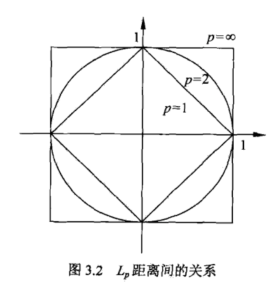
\includegraphics[width=0.8\linewidth]{pic/distances_of_lp}
	
	上图给出了二维空间中p取不同的值时,与原点的\(L_p\)距离为1的点的图形
	
	\textbf{k值的选择:}如果选择较小的k值,就相当于用较小的领域中的训练实例进行预测,学习的近似误差(approximation error)会减小,只有与输入实例较近的训练实例才会对预测结果起作用,但缺点是学习的估计误差(estimation error)会增大,预测结果会对近邻的实例点非常敏感。如果邻近的实例点恰巧是噪声,预测就会出错。
	
	换句话说,k值的减小意味着整体模型变复杂,容易发生过拟合。
	
	如果选择较大的k值,就相当于用较大的邻域的训练实例进行预测。k值的增大意味着整体的模型变简单。
	
	\textbf{分类决策规则:} 决策规则往往是多数表决(majority voting rule),即由输入实例的k个邻近的训练实例中的多数类决定输入实例的类。
	
	\subsection{k近邻法的实现}

	考虑如果对训练数据进行快速k近邻搜索
	
	\textbf{构造kd树}	
	
	kd树是一种对k维空间中的实例点进行存储以便对其进行快速检索的树形数据结构。kd树是二叉树,表示对k维空间的一个划分。构造kd树相当于不断地用垂直于坐标轴的超平面将k维空间切分,构成一系列的k维超矩形区域。kd树的每个结点对应于一个k维超矩形区域。
	
	\section{朴素贝叶斯法}
	
	朴素贝叶斯法是基于贝叶斯定理与特征条件独立假设的分类方法。对于给定的训练数据集,首先是基于特征条件独立假设学习输入/输出的联合概率分布,然后基于此模型,对给定的输入x,利用贝叶斯定理求出后验概率最大的输出y
	
	\subsection{朴素贝叶斯法的学习和分类}
	
	设输入空间\(X \subseteq R^n\)为n维向量的集合,输出空间为类标记集合\(Y = \{c_1, c_2,...,c_k\}\)。输入为特征向量\(x \in X\), 输出为类标记\(y \in Y\).X是定义在输入空间X上的随即向量,Y是定义在输出空间Y上的随机变量。P(X, Y)是X和Y的联合分布概率。训练数据集
	
	\[T = \{(x_1, y_1),(x_2, y2),...,(x_N, y_N)\}\]
	
	由P(X, Y)独立同分布产生。
	
	朴素贝叶斯法通过训练数据集学习联合概率分布P(X, Y).具体学习以下先验概率分布以及条件概率分布。
	
	先验概率分布:
	
	\[P(Y = c_k), k = 1, 2, ..., K\]
	
	条件概率分布:
	
	\[P(X = x|Y = c_k) = P(X^{(1)} = x^{(1)},...,X^{(n)} = x^{(n)}|Y = c_k), k = 1,2,...,K\]
	
	{\color{red}朴素贝叶斯法对条件概率分布作了条件独立性的假设}。即:
	
	\begin{align}
	P(X = x|Y = c_k) = P(X^{(1)} = x^{(1)},...,X^{(n)} = x^{(n)}|Y = c_k)\nonumber \\
						     = \prod_{j=1}^{n}P(X^{(j)} = x^{(j)} | Y = c_k)
	\end{align}
	
	对给定的输入x,通过学习到的模型计算后验概率分布\(P(Y=c_k|X = x)\),将后验概率最大的类作为x的类输出
	
	\[P(Y=c_k|X=x) = \frac{P(X=x|Y=c_k)P(Y=c_k)}{\sum_{k}P(X=x|Y=c_k)P(Y=c_k)}\]

	将(1)式代入上式得
	
	\[P(Y=c_k|X=x)=\frac{P(Y=c_k)\prod_{j}P(X^{(j)}=x^{(j)}|Y=c_k)}{\sum_{k}P(Y=c_k)\prod_{j}P(X^{(j)}=x^{(j)}|Y=c_k)}\]
	
	于是朴素贝叶斯分类器可表示为:
	
	\[y=f(x)=\arg \max_{c_k}\frac{P(Y=c_k)\prod_{j}P(X^{(j)}=x^{(j)}|Y=c_k)}{\sum_{k}P(Y=c_k)\prod_{j}P(X^{(j)}=x^{(j)}|Y=c_k)}\]
	
	上式中分母对所有\(c_k\)相同,所以:
	
	\[y=f(x)=\arg \max_{c_k} P(Y=c_k)\prod_{j}P(X^{(j)}=x^{(j)}|Y=c_k)\]
	
	\subsection{朴素贝叶斯法的参数估计}
		
	在朴素贝叶斯法中,学习意味着估计\(P(Y=c_k)\)和\(P(X^{(j)}=x^{(j)}|Y=c_k)\).可以应用极大似然估计法估计相应的概率。
	
	先验概率\(P(Y=c_k)\)的极大似然估计是:
	
	\[P(Y=c_k)=\frac{\sum\limits_{i=1}^{N}I(y_i=c_k)}{N}, k=1,2,...,K\]
	
	设第j个特征\(x^{(j)}\)可能取值的集合\(\{a_{j1},a_{j2},...,a_{jS_j}\}\),条件概率\(P(X^{(j)}|Y=c_k)\)的极大似然估计
	
	\[P(X^{(j)}=a_{jl}|Y=c_k)=\frac{\sum\limits_{i=1}^{N}I(x_i^{(j)} = a_{jl},y_i=c_k)}{\sum\limits_{i=1}^{N}I(y_i=c_k)}\]
	
	\[j=1,2,...,n; l=1,2,...,S_j; k=1,2,...,K\]
	
	式中,\(x_i^{(j)}\)是第i个样本的第j个特征;\(a_{(ij)}\)是第j个特征可能取得第l个值,I是指示函数
	
	\textbf{朴素贝叶斯算法}

	输入:训练数据\(T = \{(x_1, y_1),(x_2, y2),...,(x_N, y_N)\}\),其中\(x_i=(x_i^{(1)},x_i^{(2)},...,x_i^{(n)})\),\(x_i^{(j)}\)是第i个样本的第j个特征,\(x_i^{(j)} \in \{a_{(j1)},a_{(j2)},...,a_{(jS_j)}\}\), \(a_{(jl)}\)是第j个特征可能取得第l个值,j=1,2,...,n, \(l=1,2,..,S_j\), \(y_i \in \{c_1, c_2,...,c_k\}\);实例x
	
	输出:实例x的分类
	
	(1)计算先验概率及条件概率
	
	\[P(Y=c_k)=\frac{\sum\limits_{i=1}^{N}I(y_i=c_k)}{N}, k=1,2,...,K\]
	
	\[P(X^{(j)}=a_{jl}|Y=c_k)=\frac{\sum\limits_{i=1}^{N}I(x_i^{(j)} = a_{jl}, y_i=c_k)}{\sum\limits_{i=1}^{N}I(y_i=c_k)}\]

	\[j=1,2,...,n; l=1,2,...,S_j; k=1,2,...,K\]	
	
	(2)对于给定的实例\(x = (x^{(1)}, x^{(2)},...,x^{(n)})^T\),计算
	
	\[P(Y=c_k)\prod_{j}P(X^{(j)}=x^{(j)}|Y=c_k), k=1,2,...,K\]
	
	(3)确定实例x的类
	
	\[y=\arg \max_{c_k} P(Y=c_k)\prod_{j=1}P(X^{(j)}=x^{(j)}|Y=c_k)\]
	
	\textbf{贝叶斯估计}
	
	用极大似然估计可能会出现所要估计的概率值为0的情况,这时会影响到后验概率的计算结果,使分类产生偏差。解决这一问题的方法是采用贝叶斯估计。
	
	\[P_\lambda(X^{(j)} = a_{jl}|Y=c_k) = \frac{\sum\limits_{i=1}^{N}I(x_i^{(j)} = a_{jl}, y_i = c_k)+\lambda}{\sum\limits_{i=1}^{N}I(y_i=c_k)+S_j\lambda}, \lambda \geq 0\]
	
	等价于在随机变量各个取值的频数上赋予一个正数\(\lambda > 0\).当\(\lambda = 0\)时就是极大似然估计。常取\(\lambda = 1\),这时成为拉普拉斯平滑(Laplace smoothing)。
	
	显然对任何的\(l=1,2,...,S_j,  k=1,2,...,K\)有
	
	\[P_\lambda(X^{(j)} = a_{jl}|Y=c_k)  > 0\]
	
	\[\sum_{l=1}^{S_j}P(X^{(j)} = a_{jl}|Y=c_k) = 1\]
	
	同样,先验概率的贝叶斯估计
	
	\[P_\lambda(Y=c_k)=\sum_{i=1}^{N}\frac{I(y_i = c_k)+\lambda}{N+K\lambda}\]
	
	
	

	
	
	
	
	
	
	
	
	
	
	
	\begin{thebibliography}{99}
		\bibitem{ref1}李航:统计学习方法
	\end{thebibliography}
	
	
	
	
\end{document}